\subsection{Type Definition}
\label{sec:IoTDSL-TD}

The first task is to provide a description of which capabilities each device included in the \IOT system possess: how each device may provide information about the environment through a \emph{sensing} operation; and how it could react and influence it through \emph{actuations}. Our framework currently requires that an advanced user that is able to reason properly about how to effectively manipulate a device and extract the relevant information, but is flexible enough to accomodate automation in the future, so that information about devices could be automatically extracted from pre-existing devices databases (either from a knowledge database the \IOT system is connected to, or from a library of \emph{off-the-shelf devices}).

%In this section, we define \IOT devices' types, \textit{i.e.} which capabilities are available to the users in terms of getting information from the environment, \textit{a.k.a.} sensing, and operating on the environment, \textit{a.k.a} actuating. In our framework, type definitions either come from an advanced user who is able to reason properly about a particular device and extract the relevant information, or from a pre-existing devices database, either being a repository the system is connected to, or a library of \textit{devices-off-the-shelf}. 

\begin{figure*}%
  \centering  
  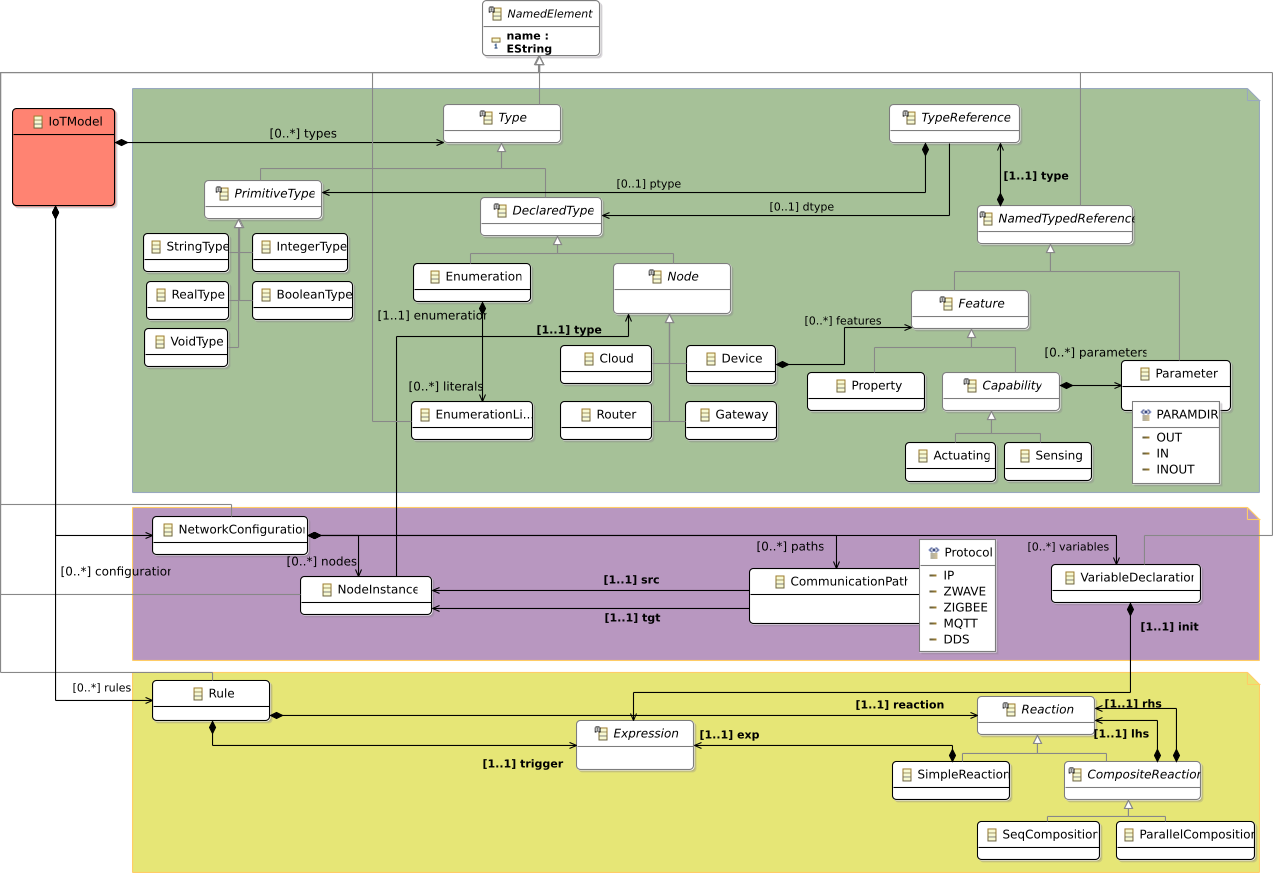
\includegraphics[width=.92\linewidth]{IoTDevice-MM.png}%
  \caption{Metamodel of \IOTDSL, separated in three concerns: \emph{Type Definition} captures devices' capabilities (top green part), \emph{Network Configuration} details how device instances are connected to each others (middle purple part), \emph{Business Rules} defines the functionalities expected from the IoT installation (bottom yellow part).}%
  \label{fig:IoTDevice-MM}%
\end{figure*}

The concepts dedicated to type definition are shown in Figure~\ref{fig:IoTDevice-MM} (green background). This part is similar to the notion of \textsf{Classifier} in \textsc{Mof}-like languages: a \textsf{Type} is either a \textsf{PrimitiveType}, or a user-defined \textsf{DeclaredType}. We distinguish between general \textsf{Gateway}s, which centralise information and processing, and \textsf{Node}s deployed in the environment and communicating with gateways, and which possess capabilities to interact with the environment. A \textsf{Capability} is basically a parameterised event that drives the node to either capture data from the environment, to act on it, or to perform both. This abstract view of an ``thing'' allows us to manipulate any device at a high abstraction level, exhibiting a clean and uniform interface for end-users based on device capabilities. Since \textsf{Node}s are \textsf{Type}s themselves, it remains possible to reference them as a parameter for the purpose of dynamic discovery across devices.

Listing~\ref{lis:RE-TypeDeclarations} illustrates how the devices in Figure~\ref{fig:scenario} are declared in \IOTDSL. Each device is introduced by the keyword \textsf{device}, possesses a name and lists capabilities that correspond to reporting events (\textsf{sensing}) or operating over the environment (\textsf{actuating}). 

\begin{table}
	\begin{minipage}[b]{.45\textwidth }%
		\begin{lstlisting}[language=iotdsl]	
gateway Middleware
device DoorDetector {
	sensing opened()
	sensing closed()
}
device MotionDetector {
	sensing moving()
}
device ToggleSwitch {
	sensing toggle();
}
		\end{lstlisting}
	\end{minipage}\hfill%
	\begin{minipage}[b]{.45\textwidth}
		\begin{lstlisting}[language=iotdsl, firstnumber=12]
		
device LightSensor {
	sensing light()
}
device LightBulb {
	actuating on()
	actuating off()
}	
device Alarm {
	actuating sound()
}
		\end{lstlisting}
	\end{minipage}
	\caption{Type declarations in \IOTDSL: capabilities as high-level events.}
	\label{lis:RE-TypeDeclarations}
\end{table}

Any IoT system should declare a special device, introduced with the keyword \textsf{gateway}, that centralises data from all devices connected to it, as we will show in Section \ref{sec:IoTDSL-NetworkConfiguration}. This device will be responsible of the event orchestration and will host the \CEP engine that embeds the implementation of the business rules. Also note that the above model is the \textit{user-defined} part of \IOTDSL. In the background, abstract events attached to all devices will need to be mapped to concrete low-level \textsc{Api}s events using a dedicated mapping language that is out of the scope of this paper.

